\newpage


\section{Background}
Computer Aided Design (CAD) software makes it easy to implement a desired logic
circuit by using a programmable logic device, such as a Field-Programmable 
Gate Array (FPGA) chip. A typical FPGA CAD flow is illustrated in Figure~\ref{fig:1}. 

\begin{figure}[H]
   \begin{center}
      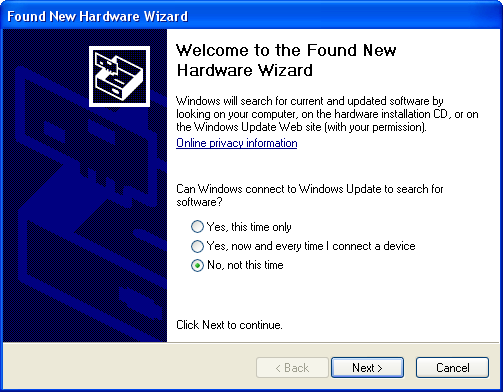
\includegraphics[scale=1]{figures/figure1.png}
   \caption{Typical CAD flow.} 
	 \label{fig:1}
	 \end{center}
\end{figure}

The CAD flow involves the following steps:
\begin{itemize}
\item {\bf Design Entry} -- the desired circuit is specified either by means of
a schematic diagram, or by using a hardware description language, 
such as Verilog or VHDL
\item {\bf Synthesis} -- the entered design is synthesized into a circuit
that consists of the logic elements (LEs) provided in the FPGA chip
\item {\bf Functional Simulation} -- the synthesized circuit is tested to
verify its functional correctness; this simulation does not take into account
any timing issues
\item {\bf Fitting} -- the CAD Fitter tool determines the placement of the LEs 
defined in the netlist into the LEs in an actual FPGA chip; it also 
chooses routing wires in the chip to make the required connections 
between specific LEs 
\item {\bf Timing Analysis} -- propagation delays along the various paths
in the fitted circuit are analyzed to provide an indication of the expected
performance of the circuit
\item {\bf Timing Simulation} -- the fitted circuit is tested to verify both
its functional correctness and timing
\item {\bf Programming and Configuration} -- the designed circuit is implemented
in a physical FPGA chip by programming the configuration switches that configure
the LEs and establish the required wiring connections
\end{itemize}

\noindent
This tutorial introduces the basic features of the Quartus Prime software. 
It shows how the software can be used to design and implement a circuit specified by
using the \typeName{} hardware description language.
It makes use of the graphical user interface to invoke the Quartus Prime commands.
Doing this tutorial, the reader will learn about:
\begin{itemize}
\item Creating a project
\item Design entry using \typeName{} code
\item Synthesizing a circuit specified in \typeName{} code
\item Fitting a synthesized circuit into an FPGA
\item Assigning the circuit inputs and outputs to specific pins on the FPGA
\item Simulating the designed circuit
\item Programming and configuring an FPGA chip
\end{itemize}
